
% ----------------------------------------------------------
% Anexos
% ----------------------------------------------------------
%
% ---
% Inicia os anexos
% ---

\begin{anexosenv}

% Imprime uma página indicando o início dos anexos
%\partanexos


\chapter{Children’s Knowledge of Abuse Questionnaire Instructions}\label{chap:CKAQInstrucoes}

My name is \rule{5.4cm}{0.15mm} and I need your help in finding out what kids your age think about different kinds of touching.

Did you know that there are at least 3 different kinds of touches? Sometimes you feel good when someone touches you - those are \underline{good} touches - like hugs and gentle pats on the back. Some touches feel \underline{bad} - like pinches and bites. They hurt or feel uncomfortable. Even kisses from someone you don’t like can be bad touches. Sometimes touches are \underline{confusing} – that’s when it’s hard to decide if they are good or bad. For example, someone you like might give you a hug, but they might squeeze too hard. You are the one to decide if a touch is good or bad, because you know how it feels for you.

The other word I want to make sure you understand is \underline{private parts}. Private parts are the areas of your bodies that your bathing suit covers. 

I’m going to ask you some questions about different kinds of touches. This is not a test for school: you won't get a mark on your report card based on how you do today. Please just answer the questions the way you think is correct. I’m going to read the questions out loud and I'd like you to write “T” if you think the answer is True, “NT” if you think the answer is Not True or False, and put a “?” if you are not sure. 

\textbf{NOTE}: A verbal administration is recommended for children of all ages, especially if the CKAQ is being used in a comparison of younger and older children whose reading skills might be different. When reading out items it is helpful to end each statement with \textbf{"IS THAT TRUE OR NOT TRUE?"} Younger children in Grades One and two (six to seven year olds) are best tested individually with the examiner recording the responses. Children in Grades Three and Four (eight to ten) do better in small groups of about six to eight and can usually record their own responses.

The CKAQ is not recommended for children in kindergarten (age five or below). CKAQ items were developed for children in elementary school and, as such, many of the items are too complex for very young children in preschool or day-care to understand.

Administration of the CKAQ takes approximately 10 to 15 minutes.

The scoring key for the revised version includes two subscales: \textbf{I for Inappropriate Touches} and \textbf{A for Appropriate Touches}. The appropriate touch items reflect appropriate interactions with another such as OK hugs. The inappropriate items reflect scenarios where there is the possibility of the child being at risk. The second subscale is in the process of being validated. 


%----------------------------------------------------------------------------XXXX


\chapter{Children’s Knowledge of Abuse \\Questionnaire Revised – III}\label{chap:CKAQ}


\noindent
\textbf{I.D. Number: \rule{5.4cm}{0.15mm} \quad Age: \rule{2.5cm}{0.15mm} \quad Boy \makebox[0pt][l]{$\square$}{}  \quad  or Girl \makebox[0pt][l]{$\square$}{}}

\vspace{1.0cm}

\noindent
\textbf{Please respond T for "True", F for "False", and DK for "Don't Know", to the following
questions:}



%\makebox[0pt][l]{$\square$}{\raisebox{0.1\height}{$\times$}} = Esse é o quadrado com o X dentro

\begin{enumerate}
	\item You always have to keep secrets.
	\item It's OK for someone you like to hug you.
	\item You can always tell who's a stranger - they look mean.
	\item Most kids like to get a kiss from their parents before they go to bed at night, so, for them, that would be a good touch.
	\item Sometimes it's OK to say no'' to a grown-up.
	\item It's OK to say ``no'' and move away if someone touches you in a way you don't like.
	\item Even if someone say that they know you, if you don't know them they're a stranger.
	\item Even hugs and tickles can turn into bad touches if they go on too long.
	\item If you fell off your bike and hurt your private parts, it would be OK for a doctor or nurse to look under your clothes.
	\item If someone touches you in a way you don't like, you should tell someone you trust.
	\item If your friend says he won't be your friend any more if you don't give him your last piece of candy, then you should give it to him.
	\item If someone touches you in a way you don't like, it's your own fault.
	\item If you don't like how someone is touching you, it's OK to say ``no''.
	\item Strangers look like ordinary people.
	\item If a grown-up tells you to do something you always have to do it.
	\item Some touches start out feeling good, then turn confusing.
	\item You can trust your feelings about whether a touch is good or bad.
	\item It's OK to have a hug from a grown-up you like.
	\item If a mean kid at school orders you to do something you had better do it.
	\item Even someone you like could touch you in a way that feels bad.
	\item A pat on the back from a teacher you like after you've done a good job at school is a good touch.
	\item You have to let grown-ups touch you whether you like it or not.
	\item If someone touches you in a way that does not feel good, you should keep on telling until someone believes you.
	\item Sometimes someone in your family might touch you in a way you don't like.
	\item Boys don't have to worry about someone touching their private parts.
	\item If you're walking down the street with your mother and she starts talking to a neighbour you have not met before, it's OK to talk with them too.
	\item If a friend's dad asks you to help him find their lost cat, you should go right away with him and help.
	\item If you won a contest for drawing the best picture in your school and a neighbour you liked gave you a quick hug to congratulate you, that would be a good touch.
	\item Most people are strangers and most strangers are nice.
	\item Someone you know, even a relative, might want to touch your private parts in a way that feels confusing.
	\item If your baby-sitter tells you to take off all your clothes but it's not time to get undressed for bed, you have to do it.
	\item If someone walks in while you are having a bath, and you feel uncomfortable, you should just keep quiet.
	\item If you get separated from your parents in a shopping mall, it's OK to ask a sales clerk or a security guard for help, even if they are strangers. 
\end{enumerate}

%----------------------------------------------------------------------------XXXX




\chapter{Model for the Evaluation of Educational GAmes}\label{chap:MEEGA}

\hspace{-1.6cm}\frame{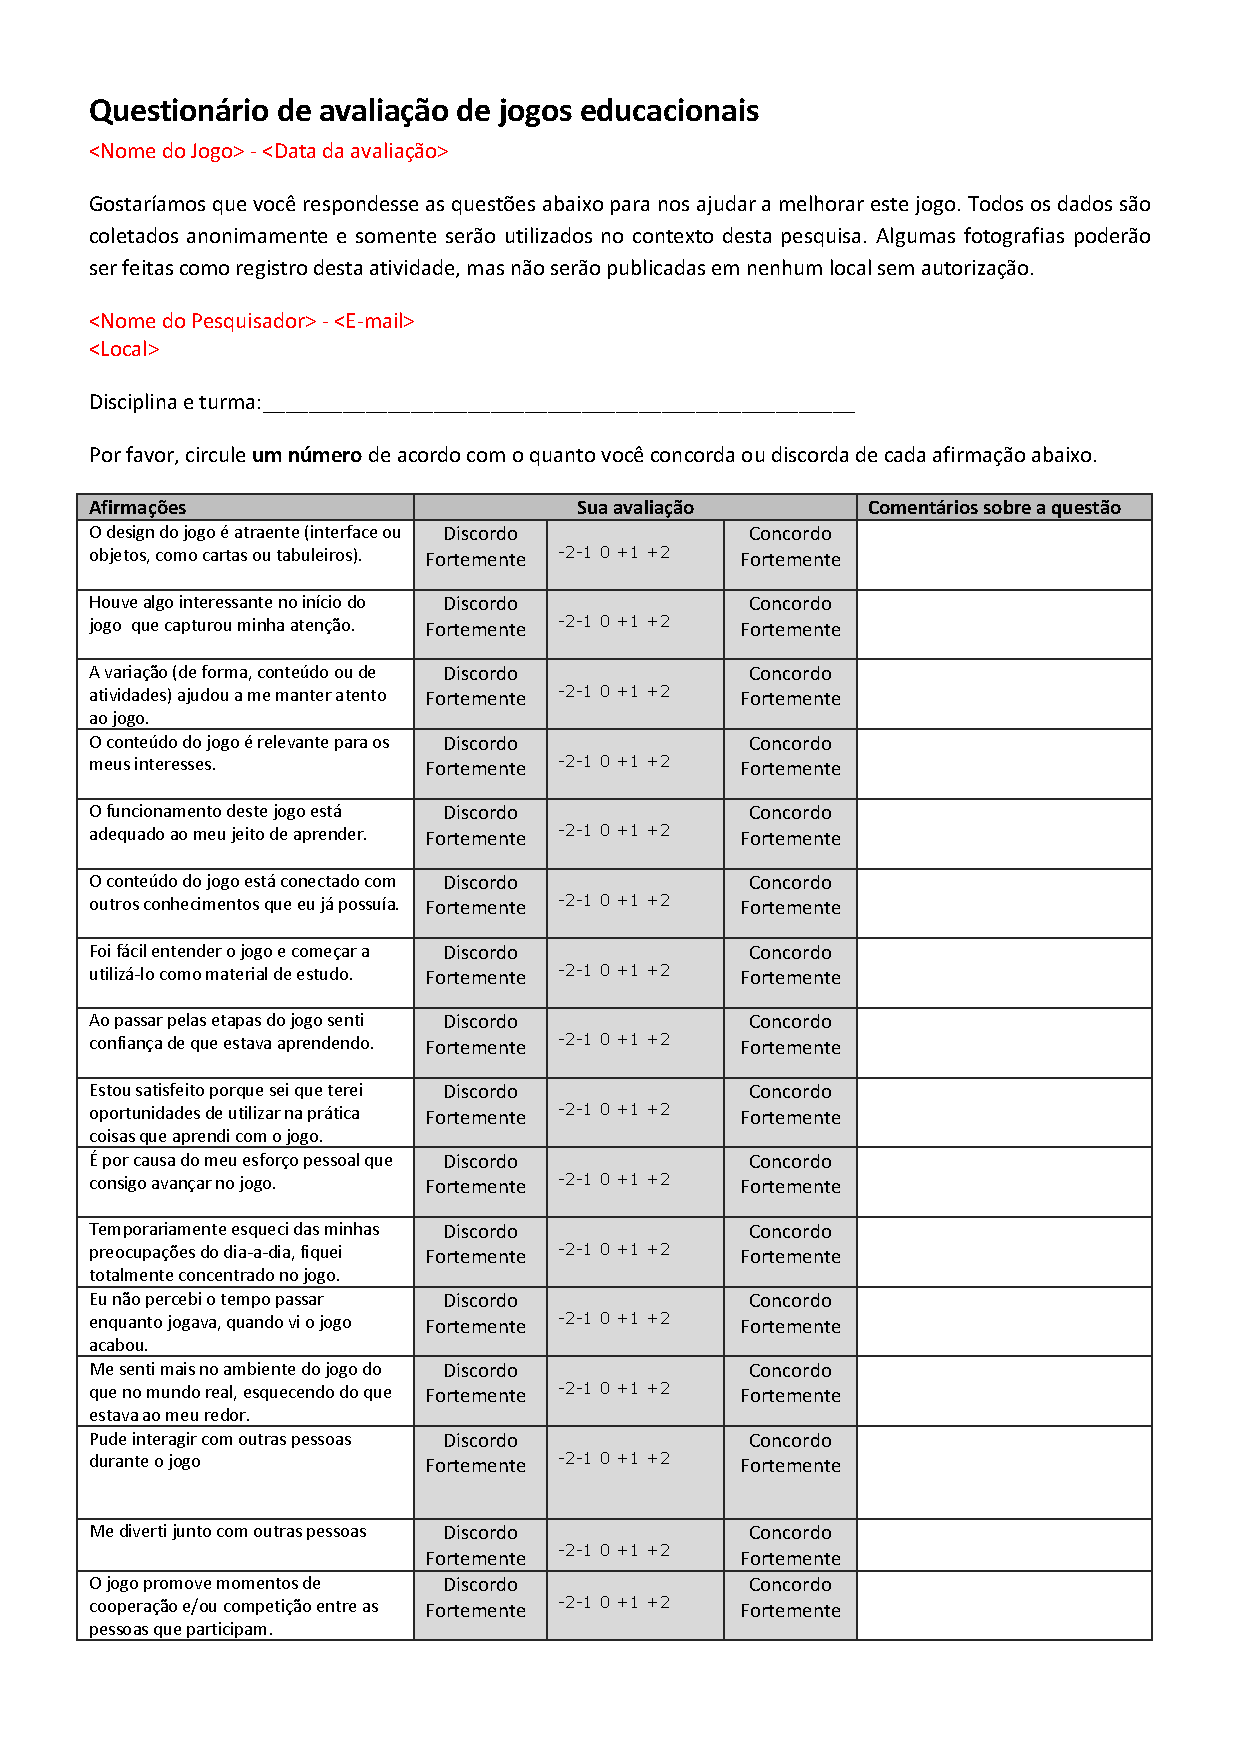
\includegraphics[page=1, width=\textwidth,height=\dimexpr\textheight-2\baselineskip\relax,keepaspectratio]{./Termos/MEEGA.pdf}}

\hspace{-1.6cm}\frame{\includegraphics[page=2, width=\textwidth,height=\dimexpr\textheight-2\baselineskip\relax,keepaspectratio]{./Termos/MEEGA.pdf}}




%----------------------------------------------------XXXXXXXXXXXXXXXXXXXXXxx



\end{anexosenv}
